
\documentclass[12pt,a4paper]{article} % Use A4 paper with a 12pt font size - different paper sizes will require manual recalculation of page margins and border positions

% Generated with LaTeXDraw 2.0.8
% Mon Jun 17 19:00:40 EDT 2013
\usepackage[usenames,dvipsnames]{pstricks}
\usepackage{epsfig}
\usepackage{pst-grad} % For gradients
\usepackage{pst-plot} % For axes
%\usepackage{marginnote} % Required for margin notes
%\usepackage{wallpaper} % Required to set each page to have a background
%\usepackage{lastpage} % Required to print the total number of pages
%\usepackage[left=1.3cm,right=4.6cm,top=1.8cm,bottom=4.0cm,marginparwidth=3.4cm]{geometry} % Adjust page margins
\usepackage{amsmath} % Required for equation customization
\usepackage{amssymb} % Required to include mathematical symbols
\usepackage{xcolor} % Required to specify colors by name
\usepackage{amsthm}
\usepackage{float}


\setlength{\parindent}{0cm} % Remove paragraph indentation
\newcommand{\tab}{\hspace*{2em}} % Defines a new command for some horizontal space


\title{Calculus and Linear Algebra Workshop Notes and Problems - Basics of Derivatives and Differentiation}
%----------------------------------------------------------------------------------------

\newtheorem{defn}{Definition}
\newtheorem{example}{Example}
\newtheorem{prop}{Proposition}
\newtheorem{exer}{Exercises}
\newtheorem{thm}{Therorem}
\begin{document}
\maketitle
\section{Preliminaries}
\subsection{Absolute Value}
In the following topics, it is helpful to think of such things as $|x -a|$ as 'distances'.  So, when you see the absolute value of a difference, you really should be thinking of the distance between the numbers on the real line.  For example, consider:
$$|(-2) - 1|$$
We can think of this expression as the distance between $-2$ and $1$ on the number line:
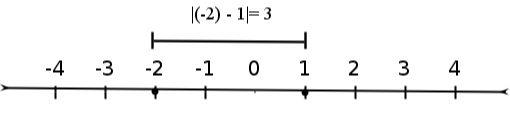
\includegraphics[]{dist.jpg}

Some useful properties of absolute value:
\begin{enumerate}
\item If $|x|\leq a$, then $-a\leq x\leq a$
\item Triangle inequality:  $|x +y| \leq |x| +|y|$
\item Reverse triangle inequality: $||x|-|y|| \leq |x-y|$
\end{enumerate}

\subsection{Functions}
Recall that a function is a rule that assigns an output value to some input value.  For example, a rule might be to take the input (a real number) and output its square (also a real number).  We can call this rule $f$ and write:
\begin{equation*}
f(x) = x^2
\end{equation*}
Mathematicians like to be clear on the input (domain) of a function and the output (range) of a function.  Because our $f$ above can take any real number and will output a real number, we say that $f$ is a real-valued function of a real variable.  That is a lot to say.  We can use a shorthand, by denoting the set of real numbers by $\mathbb{R}$.  We then write:
\begin{equation}
f:\mathbb{R}\rightarrow \mathbb{R}
\end{equation}
This says the same thing as '$f$ is a real-valued function of a real variable', but it is shorter, and we may read it as '$f$ is a function from $\mathbb{R}$ to $\mathbb{R}$'.  You will encounter functions on other sets, for example, $\mathbb{N}$ - the natural numbers, $\mathbb{Z}$ - the integers, etc.  We will mostly focus on real functions of real variables for the purposes of these notes. 
\section{Derivatives}
Recall the following definition:
\begin{defn}
Let $f:\mathbb{R}\rightarrow\mathbb{R}$ and suppose that the following limit exists:
$$\lim_{\Delta x\rightarrow 0} \frac{f(x+\Delta x) - f(x)}{\Delta x}$$
Then we say that $f$ is \emph{differentiable} at $x$, and the limit is the \emph{derivative of} $f$ \emph{at} $x$.
\end{defn}
The derivative as defined above is the 'limit of the difference quotient'.  In English, that means that the derivative of $f$ is the limit of the slopes of secant lines through the points $(x+\Delta x,f(x+\Delta x)$ and $(x,f(x))$.  As usual, a picture conveys meaning much more easily than words:
\begin{figure}[H]
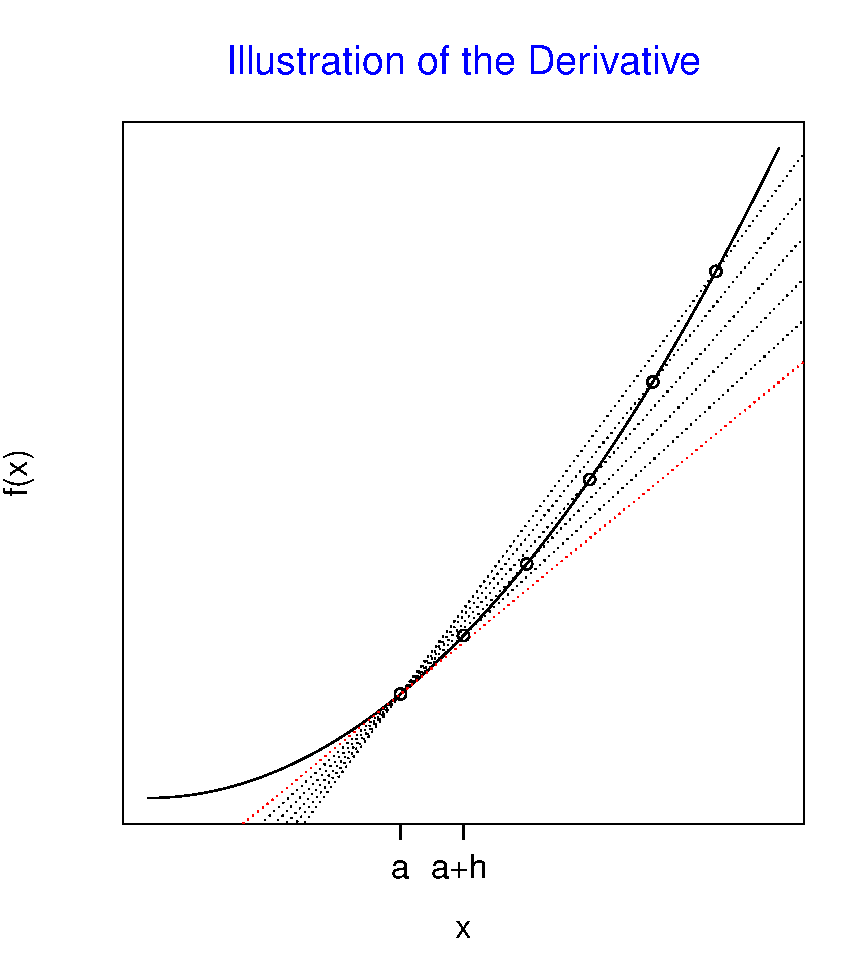
\includegraphics[height=3in]{derivative.pdf}
\end{figure}
As $\Delta x$ gets smaller, the secant line converges to the tangent line.  The value of the limit of the difference quotient is the slope of the tangent line to the curve at a point.  This value may be interpreted as an 'instantaneous' rate of change.  Later, we will discuss optimization of functions (finding maxima and minima).  We will make use of the notion that when the derivative is positive, the function is increasing.  When it is negative, the function is decreasing.\\
Note that we have not actually formally defined the 'limit' of a function at a point. For now, we will rely on our intuitive notion that the limit of a function at a point (say, $x=a$) is a value that the function achieves as $x$ gets closer to $a$ from either side. Later, we will formally define limits and proved them, using the formal definition ($\epsilon-\delta$ proofs).\\
Also note that we may consider the derivative as a \emph{function} or as a single value. In other words, we may consider the above limit at all $x$ in the domain of $f$ (for which the limit exists), or we may just want to consider the derivative at a single point. These two situations will look very much the same, as we will usually compute the derivative function and then evaluate it at a particular point.\\
If the limit exists for a particular point $x=a$, we say that the function is \emph{differentiable} at $a$. If the limit exists for all values of $x$ in the domain of $f$, we say that $f$ is differentiable.\\

A standard differential calculus course will usually begin with the limit definition of the derivative, have you use it to compute a few simple examples, and then will prove formulas that provide essential shortcuts for the purpose of computation. We will skip the first part (in the interest of time), and move right on to the formulas. You are encouraged to find a text (or ask me!) to review such examples and proofs. 
\subsection{Computing Derivatives}
The following is a summary of some important differentiation formulas:
\begin{itemize}
\item Let $f(x) = c$, where $c$ is a constant. Then $f'(x)=0$.
\item Let $f(x) = x^n$, where $n$ is \emph{any real number}. $f'(x) = nx^{n-1}$. Note that $f(x)$ and/or $f'(x)$ may not be defined at $x=0$.
\item Linearity. Let $f(x)$ and $g(x)$ be differentiable functions and let $c$ be a constant:
$$\left(cf(x)\right)' = cf'(x)$$
$$\left(f(x)+g(x)\right)' = f'(x) + g'(x)$$
\item Product Rule. Let $f(x)$ and $g(x)$ be differentiable functions.
$$\left(f(x)g(x)\right)' = f'(x)g(x) + f(x)g'(x)$$
\item Quotient Rule. Let $f(x)$ and $g(x)$ be differentiable functions. For any $x$ such that $g(x)\neq0$
$$\left(\frac{f(x)}{g(x)}\right)' = \frac{f'(x)g(x)-f(x)g'(x)}{\left(g(x)\right)^2}$$
\item Chain Rule
$$\left(f(g(x))\right)' = f'(g(x))g'(x)$$
\end{itemize}
Derivatives of some special functions:
\begin{itemize}
\item $$\frac{d}{dx}\log(x) = \frac1{x}$$
\item $$\frac{d}{dx}\sin(x) = \cos(x)$$
\item $$\frac{d}{dx}\cos(x) = -\sin(x)$$
\item $$\frac{d}{dx}e^x = e^x$$
\end{itemize}
Now, let's put these together and do some computations. Compute derivatives of the following functions:
\begin{enumerate}
\item $$f(x) = 7x^5+4x^3-6x+2$$
\item $$\frac{x^3+6}{x^2}$$
\item $$\cos(x^3)$$
\item $$e^{-x^2/2}$$
\item $$x^5\log(\cos(x))$$

\end{enumerate}
\end{document}